%%%%%%%%%%%%%%%%%%%%%%%%%%%%%%%%%%%%%%%%%%%%%%%%%%%%%%%%%%%%
%%% LaPreprint: PREPRINT TEMPLATE
%%%%%%%%%%%%%%%%%%%%%%%%%%%%%%%%%%%%%%%%%%%%%%%%%%%%%%%%%%%%

% Here I could talk about what one should do in this document.
% Instead I'll refer you to the explore on your own and check the Github Repo. :-)
% Line spacing is 1.2 by default (can't be smaller).

%%%%%%%%%%%%%%%%%%%%%%%%%%%%%%%%%%%%%%%%%%%%%%%%%%%%%%%%%%%%
%%% PREAMBLE
%%%%%%%%%%%%%%%%%%%%%%%%%%%%%%%%%%%%%%%%%%%%%%%%%%%%%%%%%%%%

% Declare document class
\documentclass[11pt,biorxiv,onehalfspacing,lineno]{lapreprint}
% Choose between "biorxiv", "medrxiv", "arxiv" and "chemrxiv". Otherwise defaults "Preprint".
% Choose between "blue" and "red" colour scheme. Defaults to "blue".
% Use the "onehalfspacing" option for 1.5 line spacing.
% Use the "doublespacing" option for 2.0 line spacing.
% Use the "lineno" option for line numbers.
% Use the "endfloat" option to place floats after the bibliography.
% Use the "secnum" option to have include numbers.

% Import packages
% \usepackage{lipsum}     % Required to insert dummy text
\usepackage[version=4]{mhchem} % For chemical notation
\usepackage{siunitx}    % For SI units
\usepackage{pdflscape}  % For putting pages in landscape mode
\usepackage{rotating}   % For rotating specific elements
\usepackage{textgreek}  % Greek symbols
\usepackage{gensymb}    % Symbols
\usepackage[misc]{ifsym} % For the \Letter symbol
\usepackage{orcidlink}  % For the \orcidlink
\usepackage{listings}   % For inserting code chunks
\usepackage{colortbl}   % For Knitr table colouring
\usepackage{tabularx}   % For making Knitr tables compatible
\usepackage{longtable}  % For multi-page tables
\usepackage{subcaption}
\usepackage{multirow}
\usepackage{snotez}     % For sidenote environments. enotez for endnotes
\usepackage{csquotes}   % For language-based quote rules (helps BiBLaTeX)
\usepackage{annotate-equations}

% Make declarations
\DeclareSIUnit\Molar{M}

% Please note that these options may affect formatting. 

%%%%%%%%%%%%%%%%%%%%%%%%%%%%%%%%%%%%%%%%%%%%%%%%%%%%%%%%%%%%
%%% BIBLIOGRAPHY
%%%%%%%%%%%%%%%%%%%%%%%%%%%%%%%%%%%%%%%%%%%%%%%%%%%%%%%%%%%%
\usepackage[			% use biblatex for bibliography
	backend=biber,      % use biber or bibtex backend
    style=authoryear,   % choose style
	natbib=true,		% allow natbib commands
	hyperref=true,	    % activate hyperref support
	alldates=year,      % only show year (not month)
    uniquename=false,   % don't add firstnames when citing multiple sources by the same author
    maxbibnames=99,     % maximum number of author names to list in bibliography before 'et al' is used instead
]{biblatex}

% Just avoiding some rogue fields that cause issues with certain styles 
\AtEveryBibitem{
    \clearfield{urlyear}
    \clearfield{urlmonth}
    \clearlist{language}
}

% Update to your bibliography file
\addbibresource{src/bibliography.bib}

%%%%%%%%%%%%%%%%%%%%%%%%%%%%%%%%%%%%%%%%%%%%%%%%%%%%%%%%%%%%
%%% ARTICLE SETUP
%%%%%%%%%%%%%%%%%%%%%%%%%%%%%%%%%%%%%%%%%%%%%%%%%%%%%%%%%%%%

% Paper title
\title{hlabud: HLA genotype analysis in R}

% Authors - you can use \orcidlink{} and \authfn{} - see contribution note
\author[ \orcidlink{0000-0002-2843-6370} 1 \Letter]{Kamil Slowikowski}
\author[ \orcidlink{0000-0001-7461-04082} 2]{Alexandra-Chloe Villani}

% Affiliations
\affil[1]{Center for Immunology and Inflammatory Diseases, Division of Rheumatology, Allergy an Immunology, Department of Medicine, Massachusetts General Hospital}
\affil[2]{Cancer Center, Massachusetts General Hospital}
\affil[3]{Broad Institute}
\affil[4]{Harvard Medical School}

% Other metadata. Feel free to add your own
%\metadata[]{\Letter\hspace{.5ex} For correspondence}{\url{https://github.com/roaldarbol/LaPreprint/issues} (MRA)}
%\metadata[\authfn{1}\authfn{2}\authfn{3}]{}{Here's a few symbols to denote contribution specifics, e.g. authors who contributed equally to the work.}
%\metadata[]{Present address}{Evolution, Behaviour and Environment, School of Life Sciences, University of Sussex, Biology Road, Brighton, BN1 9RH, United Kingdom}
%\metadata[]{Data availability}{Data availability statement. Preprocessed data could be available e.g. on \href{https://zenodo.org/}{Zenodo}.}
%\metadata[]{Funding}{MRA was supported by funding from the Leverhulme Foundation. The funders had no role in the template design or decision to publish.}
\metadata[]{}{
\begin{minipage}{0.3\textwidth}%
\vspace{-32.5em}
\hspace{-0.2\textwidth}

\includegraphics[width=\textwidth]{src/figures/logo.eps}%
\end{minipage}
}


% Surname of the lead author(s) for the running footer
\leadauthor{Slowikowski}
\shorttitle{hlabud}

%%%%%%%%%%%%%%%%%%%%%%%%%%%%%%%%%%%%%%%%%%%%%%%%%%%%%%%%%%%%
%%% ARTICLE START
%%%%%%%%%%%%%%%%%%%%%%%%%%%%%%%%%%%%%%%%%%%%%%%%%%%%%%%%%%%%

\begin{document}
\maketitle
\begin{abstract}
\textbf{Summary:} The human leukocyte antigen (HLA) genes have more associations with human diseases than any other genes, and there are thousands of different HLA alleles in the human population.
Data for all known HLA genotypes are curated in the international ImMunoGeneTics (IMGT) database, and allele frequencies for each HLA allele across human populations are available in the Allele Frequency Net Database (AFND).
Our open-source R package \textit{hlabud} accesses HLA data from IMGT and AFND, and supports further analysis such as HLA divergence calculation, fine-mapping analysis of amino acid (or nucleotide) positions, and low-dimensional embedding.

\textbf{Availability:} Source code and documentation are available at \href{https://github.com/slowkow/hlabud}{github.com/slowkow/hlabud}

\textbf{Contact:} \href{mailto:kslowikowski@mgh.harvard.edu}{kslowikowski@mgh.harvard.edu}

\textbf{Keywords:} immunoinformatics, genetics, immunology, HLA

\end{abstract}
\section{Introduction} \label{intro}

Human leukocyte antigen (HLA) genes encode the proteins that enable cells to display antigens to other cells, which is one mechanism for immune recognition of pathogens such as bacteria and viruses.
Geneticists have identified thousands of variants (e.g. single nucleotide polymorphisms) in the human genome that are associated with hundreds of different diseases and phenotypes Kennedy2017. HLA genes have a greater number of disease associations than any other genes.

HLA nomenclature consists of allele names like \textit{HLA*01:01} and \textit{HLA*02:01} to indicate the genotype of an individual in a study Marsh2010.
Each allele name corresponds to a haplotype that contains multiple mutations at different positions throughout the entire length of the gene sequence.
It is difficult to estimate the similarity of two alleles solely from the allele names: any two alleles might differ by one or more nucleotide or amino acid residues.
Any encoding of genotype data that is ambiguous regarding nucleotide or amino acid positions is not ideal for statistical analysis, because some positions might contain more information than others.

Researchers have developed many software tools for calling HLA genotypes (diagram) with high accuracy from DNA-seq or RNA-seq next-generation sequencing reads Claeys2023, so there are opportunities to use this type of data for HLA association studies.
Providers of HLA typing services often report genotypes with the traditional HLA allele names (i.e. \textit{HLA*01:01}) instead of reporting alleles at specific nucleotide positions (diagram), and most software tools produce outputs that follow this convention of reporting allele names.

In contrast to allele-level analysis, fine-mapping analysis associates a phenotype with each amino acid (or nucleotide) at each position.
Many amino acid residues at specific loci have been associated with human diseases and blood protein levels Krishna2023.
Published amino acid associations represent opportunities for experimental validation that could advance understanding of the disease-associated mechanisms related to HLA proteins.

Results from fine-mapping analysis can be interpreted in the context of the protein structures that are affected by the associated amino acid positions.
We might have different hypotheses about the function of a mutation in the peptide binding groove than a mutation in the interior region of the protein.

To facilitate HLA fine-mapping, we developed \textit{hlabud}, a free and open-source R package that downloads data from the IMGT/HLA database Robinson2020 and automatically creates amino acid (or nucleotide) position matrices that are ready for analysis (diagram).
\textit{hlabud} functions return simple lists, where each item in the list is a matrix or a data frame.
This design makes it easy to integrate \textit{hlabud} with any downstream R packages for data analysis or visualization.

%\section{Methods \& Materials} \label{methods}

\subsection{Behavioural setup}
\lipsum[2]

\subsection{Electrophysiological setup}
\lipsum[2] 



%Use \verb|\section| and \verb|\subsection| commands to organize your document. \LaTeX{} handles all the formatting automatically. Use \verb|\label| and \verb|\nameref| commands for cross-referencing sectional headings: the usual \verb|\ref| will not work, as this template uses unnumbered sectional headings. \par
%\lipsum[2]

%\subsection{Figures and Tables}
%Use the table and tabular commands for basic tables --- see \TABLE{example}, for example. For tables, I recommend that you use a separate .tex file for each table and insert it using \verb|\input{mytable.tex}|.

%You can upload a figure (JPEG, PNG or PDF) using the project menu. To include it in your document, use the \verb|\includegraphics| command as in the code for \FIG{view}. 

%Really wide figures or tables, that take up the entire page, including the gutter space: use \verb|\begin{fullwidth}...\end{fullwidth}| as in \FIG{fullwidth}. And sometimes you may want to use feature boxes like \BOX{simple}.

\begin{figure}
    \begin{fullwidth}
    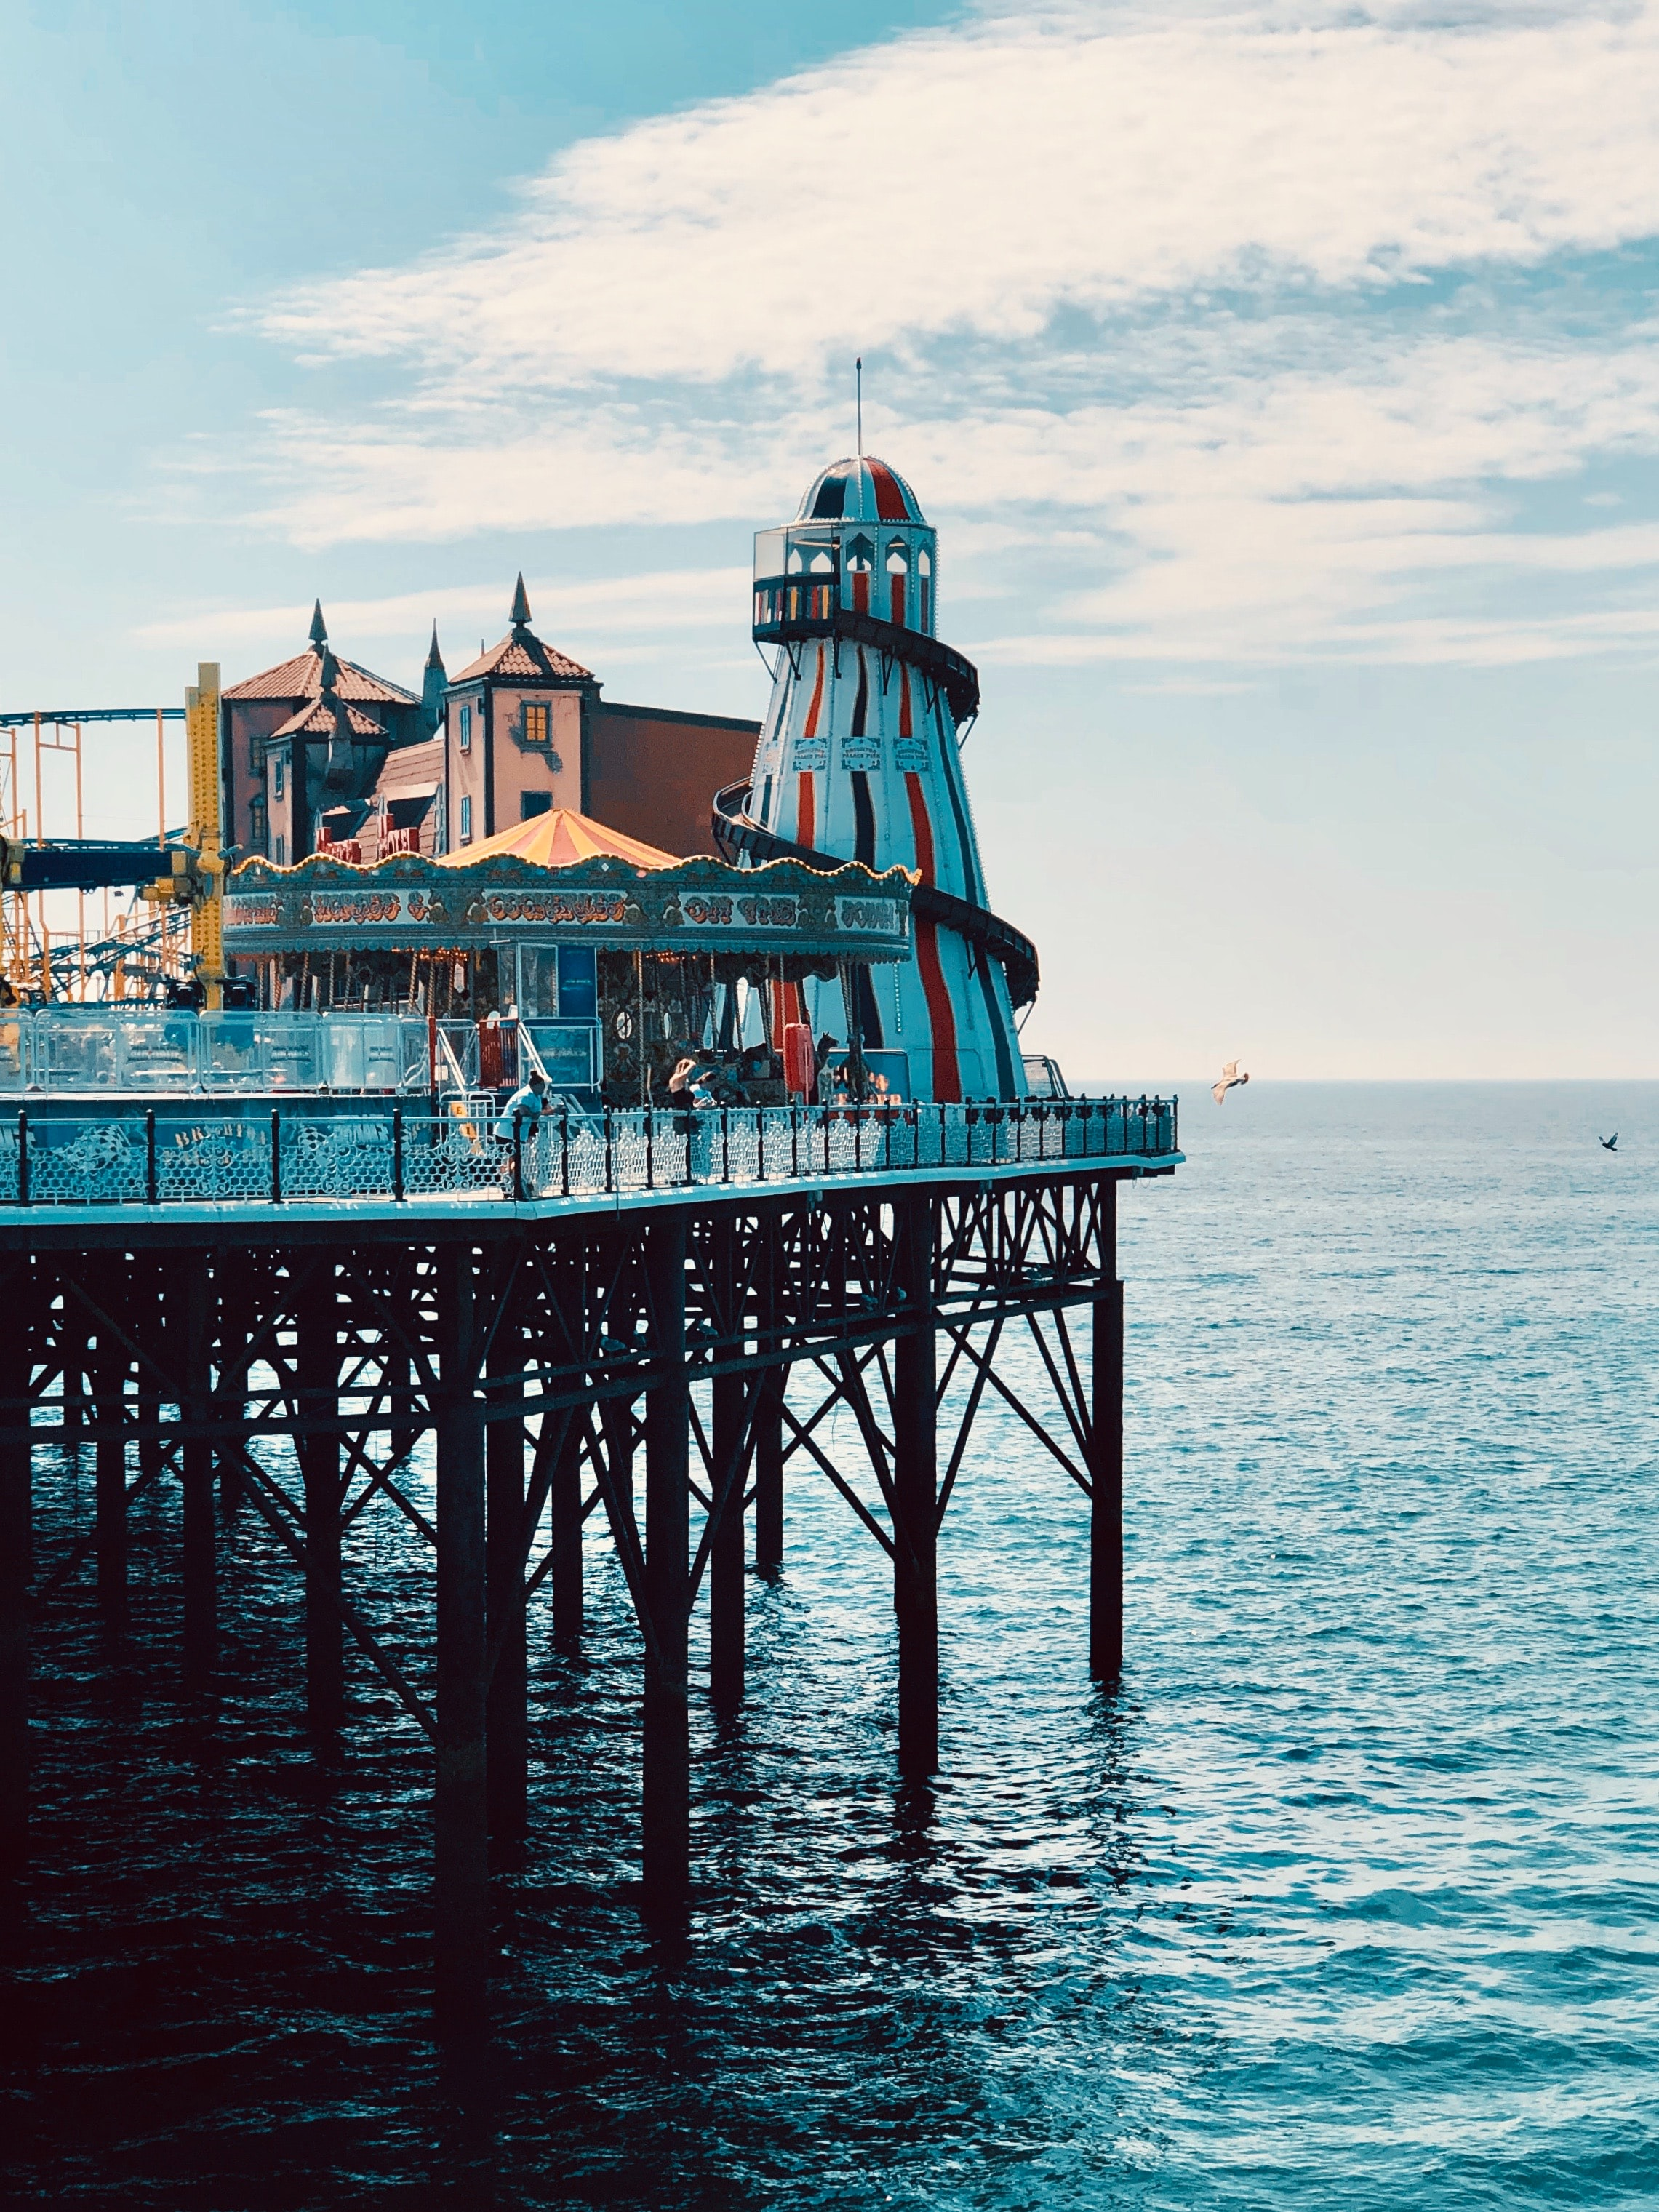
\includegraphics[width=0.65\textheight]{src/figures/brighton.jpeg}
    \caption{\textbf{Photo of lovely Brighton by \href{https://unsplash.com/es/@sanekovs?utm_source=unsplash&utm_medium=referral&utm_content=creditCopyText"}{Alex Ovs} on \href{https://unsplash.com/s/photos/brighton?utm_source=unsplash&utm_medium=referral&utm_content=creditCopyText}{Unsplash}.
    } As a very wide figure that takes up the entire page, including the gutter space.}
    \label{fig:fullwidth}
    \figsupp{There is no limit on the number of Figure Supplements for any one primary figure. Each figure supplement should be clearly labelled, Figure 1--Figure Supplement 1, Figure 1--Figure Supplement 2, Figure 2--Figure Supplement 1 and so on, and have a short title (and optional legend). Figure Supplements should be referred to in the legend of the associated primary figure, and should also be listed at the end of the article text file.}{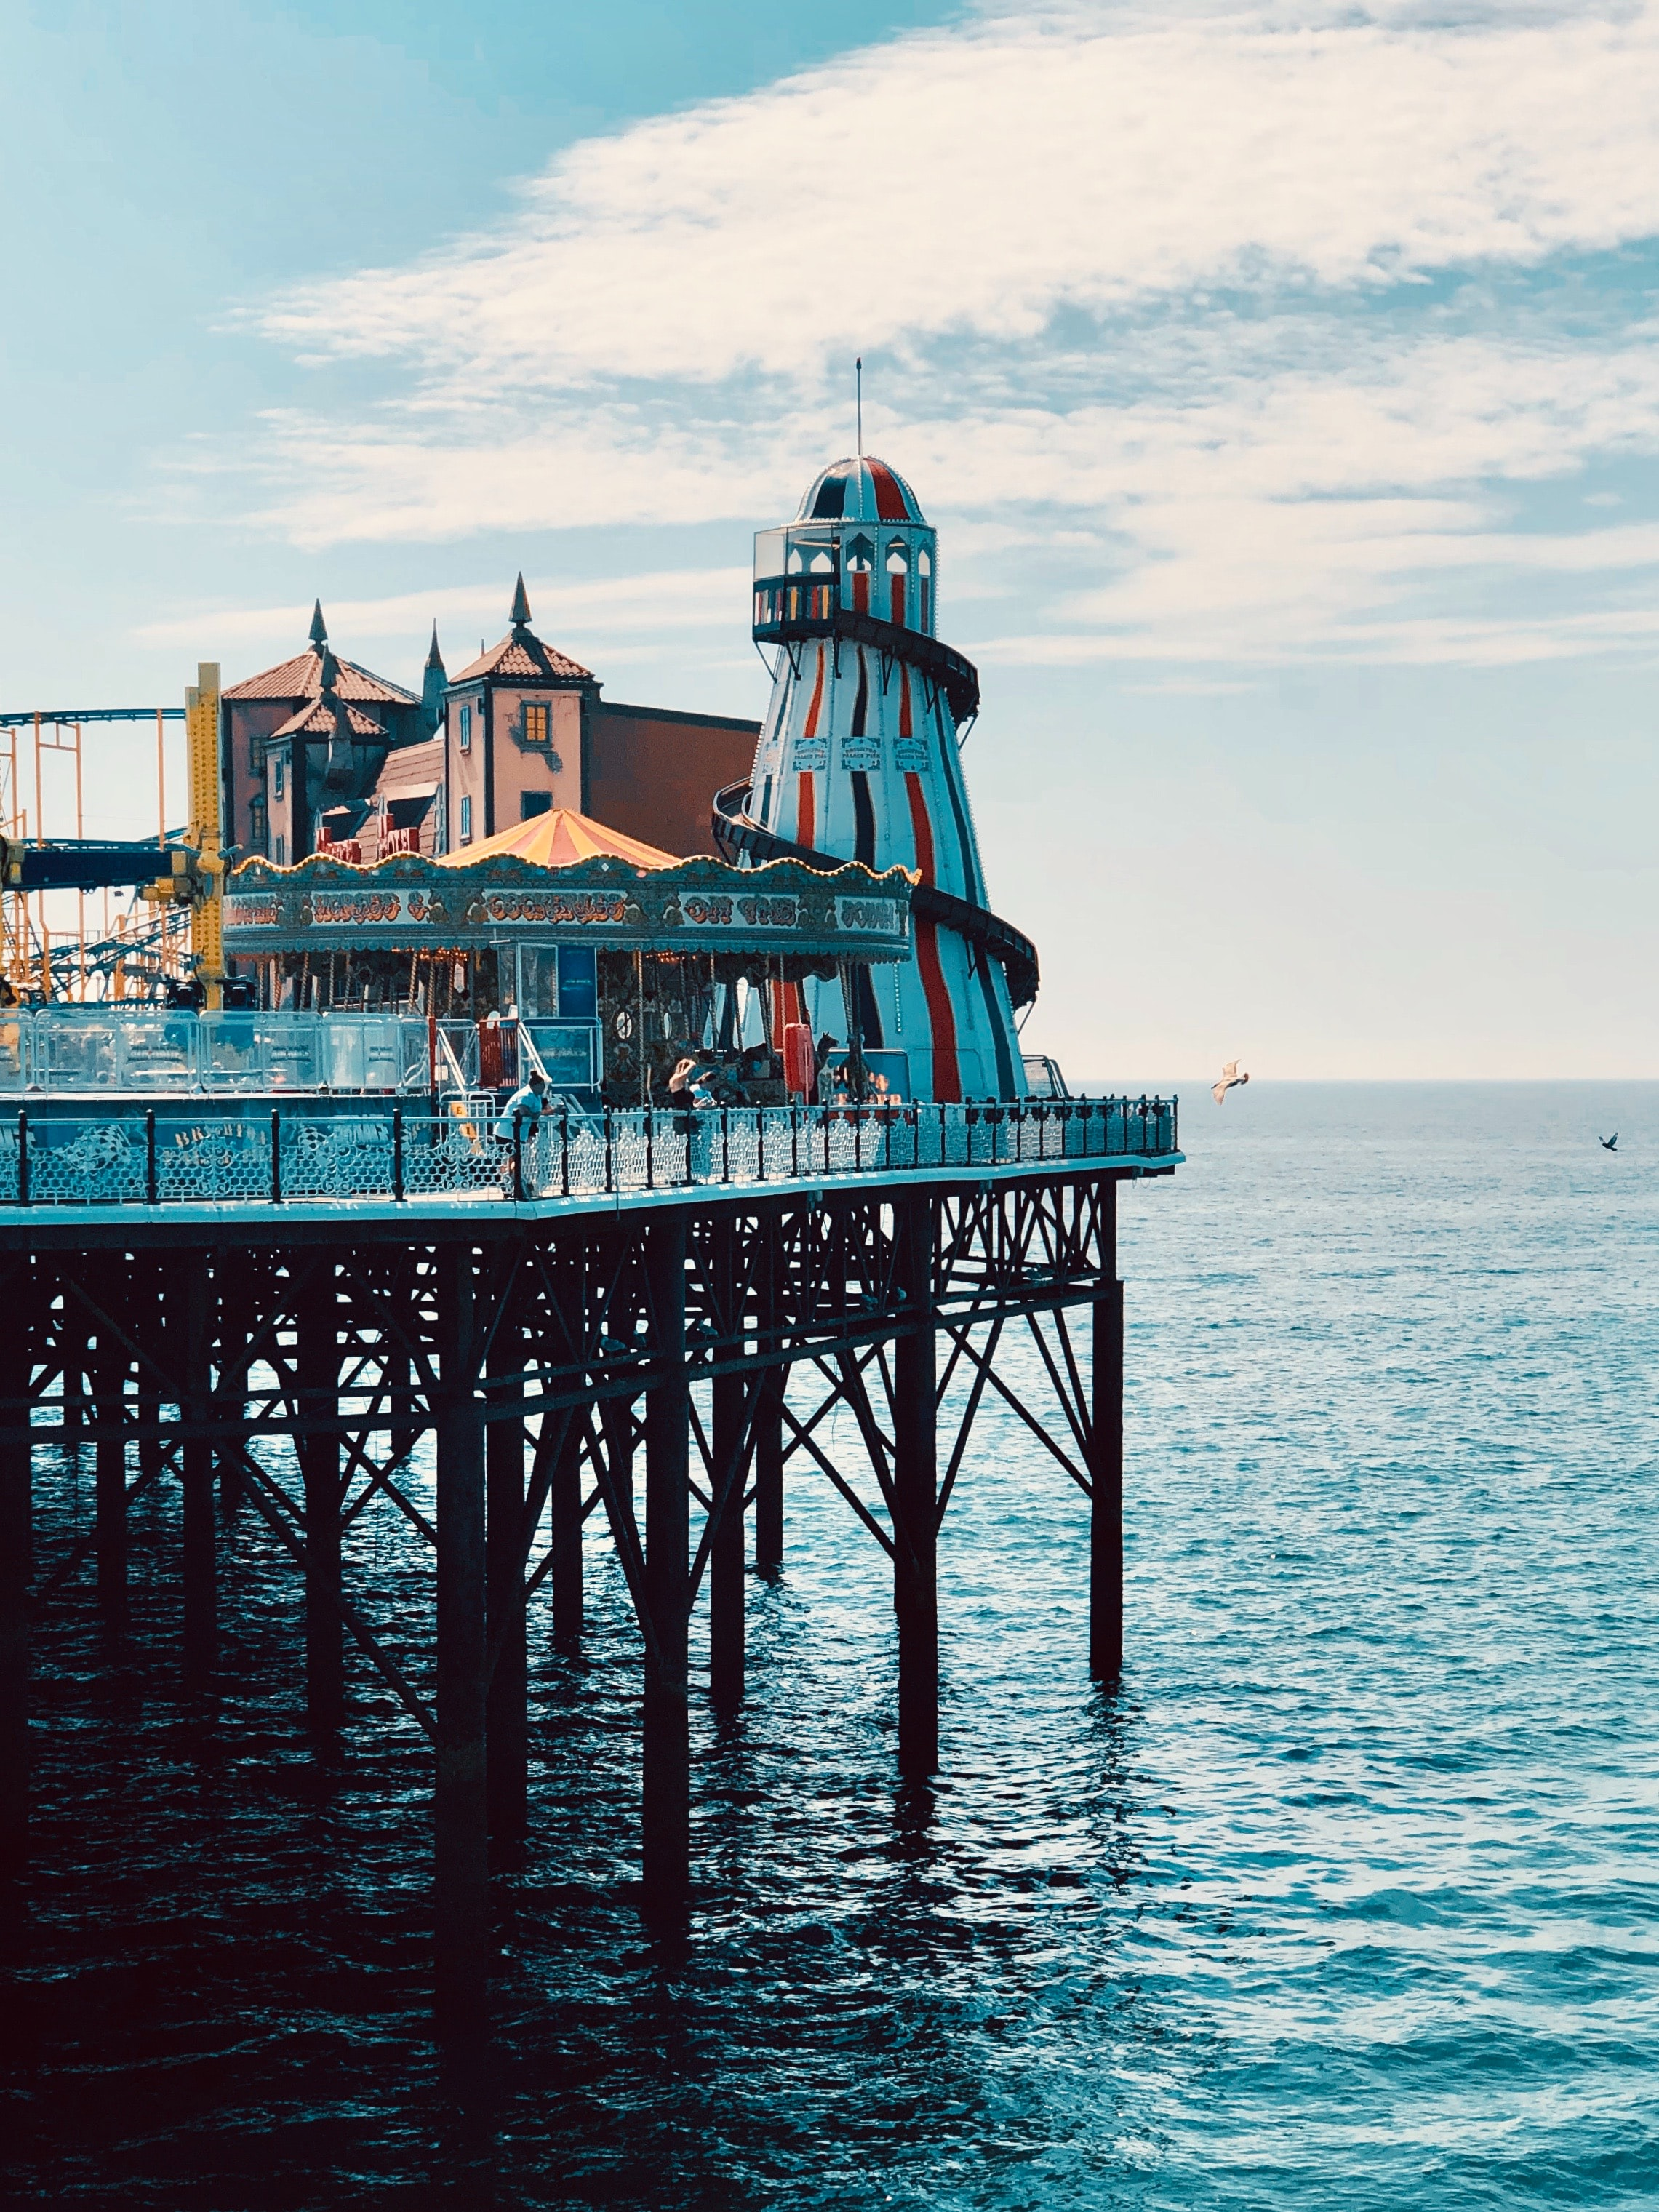
\includegraphics[width=5cm]{src/figures/brighton.jpeg}}
    \end{fullwidth}
\end{figure}

\subsection{Citations and notes}

LaTeX formats citations and references automatically using the bibliography records in your .bib file. Use the \verb|\cite| command for an inline citation, like \cite{Pooley2021}, and the \verb|\parencite| command for a citation in parentheses \parencite{Brembs2021}. Side notes makes good use of the empty margin and can be used ewith the \verb|\sidenote| command. \sidenote{This is a sidenote made with the \textbackslash sidenote package. \lipsum[1]}


\begin{featurebox}
\caption{This is an example feature box}
\label{box:simple}
This is a feature box. It floats!
\medskip

\includegraphics[width=5cm]{example-image}
\featurefig{`Figure' and `table' captions in feature boxes should be entered with \texttt{\textbackslash featurefig} and \texttt{\textbackslash featuretable}. They're not really floats.}

\lipsum[1]
\end{featurebox}

\subsection{Mathematics}

\LaTeX{} is great at typesetting mathematics $abc$. Let $X_1, X_2, \ldots, X_n$ be a sequence of independent and identically distributed random variables with $\text{E}[X_i] = \mu$ and $\text{Var}[X_i] = \sigma^2 < \infty$, and let
\begin{equation}
\label{eq:CLT}
S_n = \frac{X_1 + X_2 + \cdots + X_n}{n}
      = \frac{1}{n}\sum_{i}^{n} X_i
\end{equation}
denote their mean. Then as $n$ approaches infinity, the random variables $\sqrt{n}(S_n - \mu)$ converge in distribution to a normal $\mathcal{N}(0, \sigma^2)$.

You can even get extra fancy and annotate your equations directly: %this uses the `annotate-equations` package. See `https://ctan.org/pkg/annotate-equations` for further info and ideas

\vspace{1.5em} 
\begin{equation}
\label{eq:CLT2}
S_n = \frac{\eqnmarkbox[blue]{a1}{X_1 + X_2 + \cdots + X_n}}{n}
      = \frac{1}{n}\sum_{i}^{n} \eqnmarkbox[purple]{a2}{X_i}
\end{equation}
\annotate[yshift=1em]{above}{a1}{independent and identically distributed random variables}
\annotate[yshift=-1em]{below,left}{a2}{a random variable}
\vspace{1.5em} 

\lipsum[3] 

\begin{figure}
    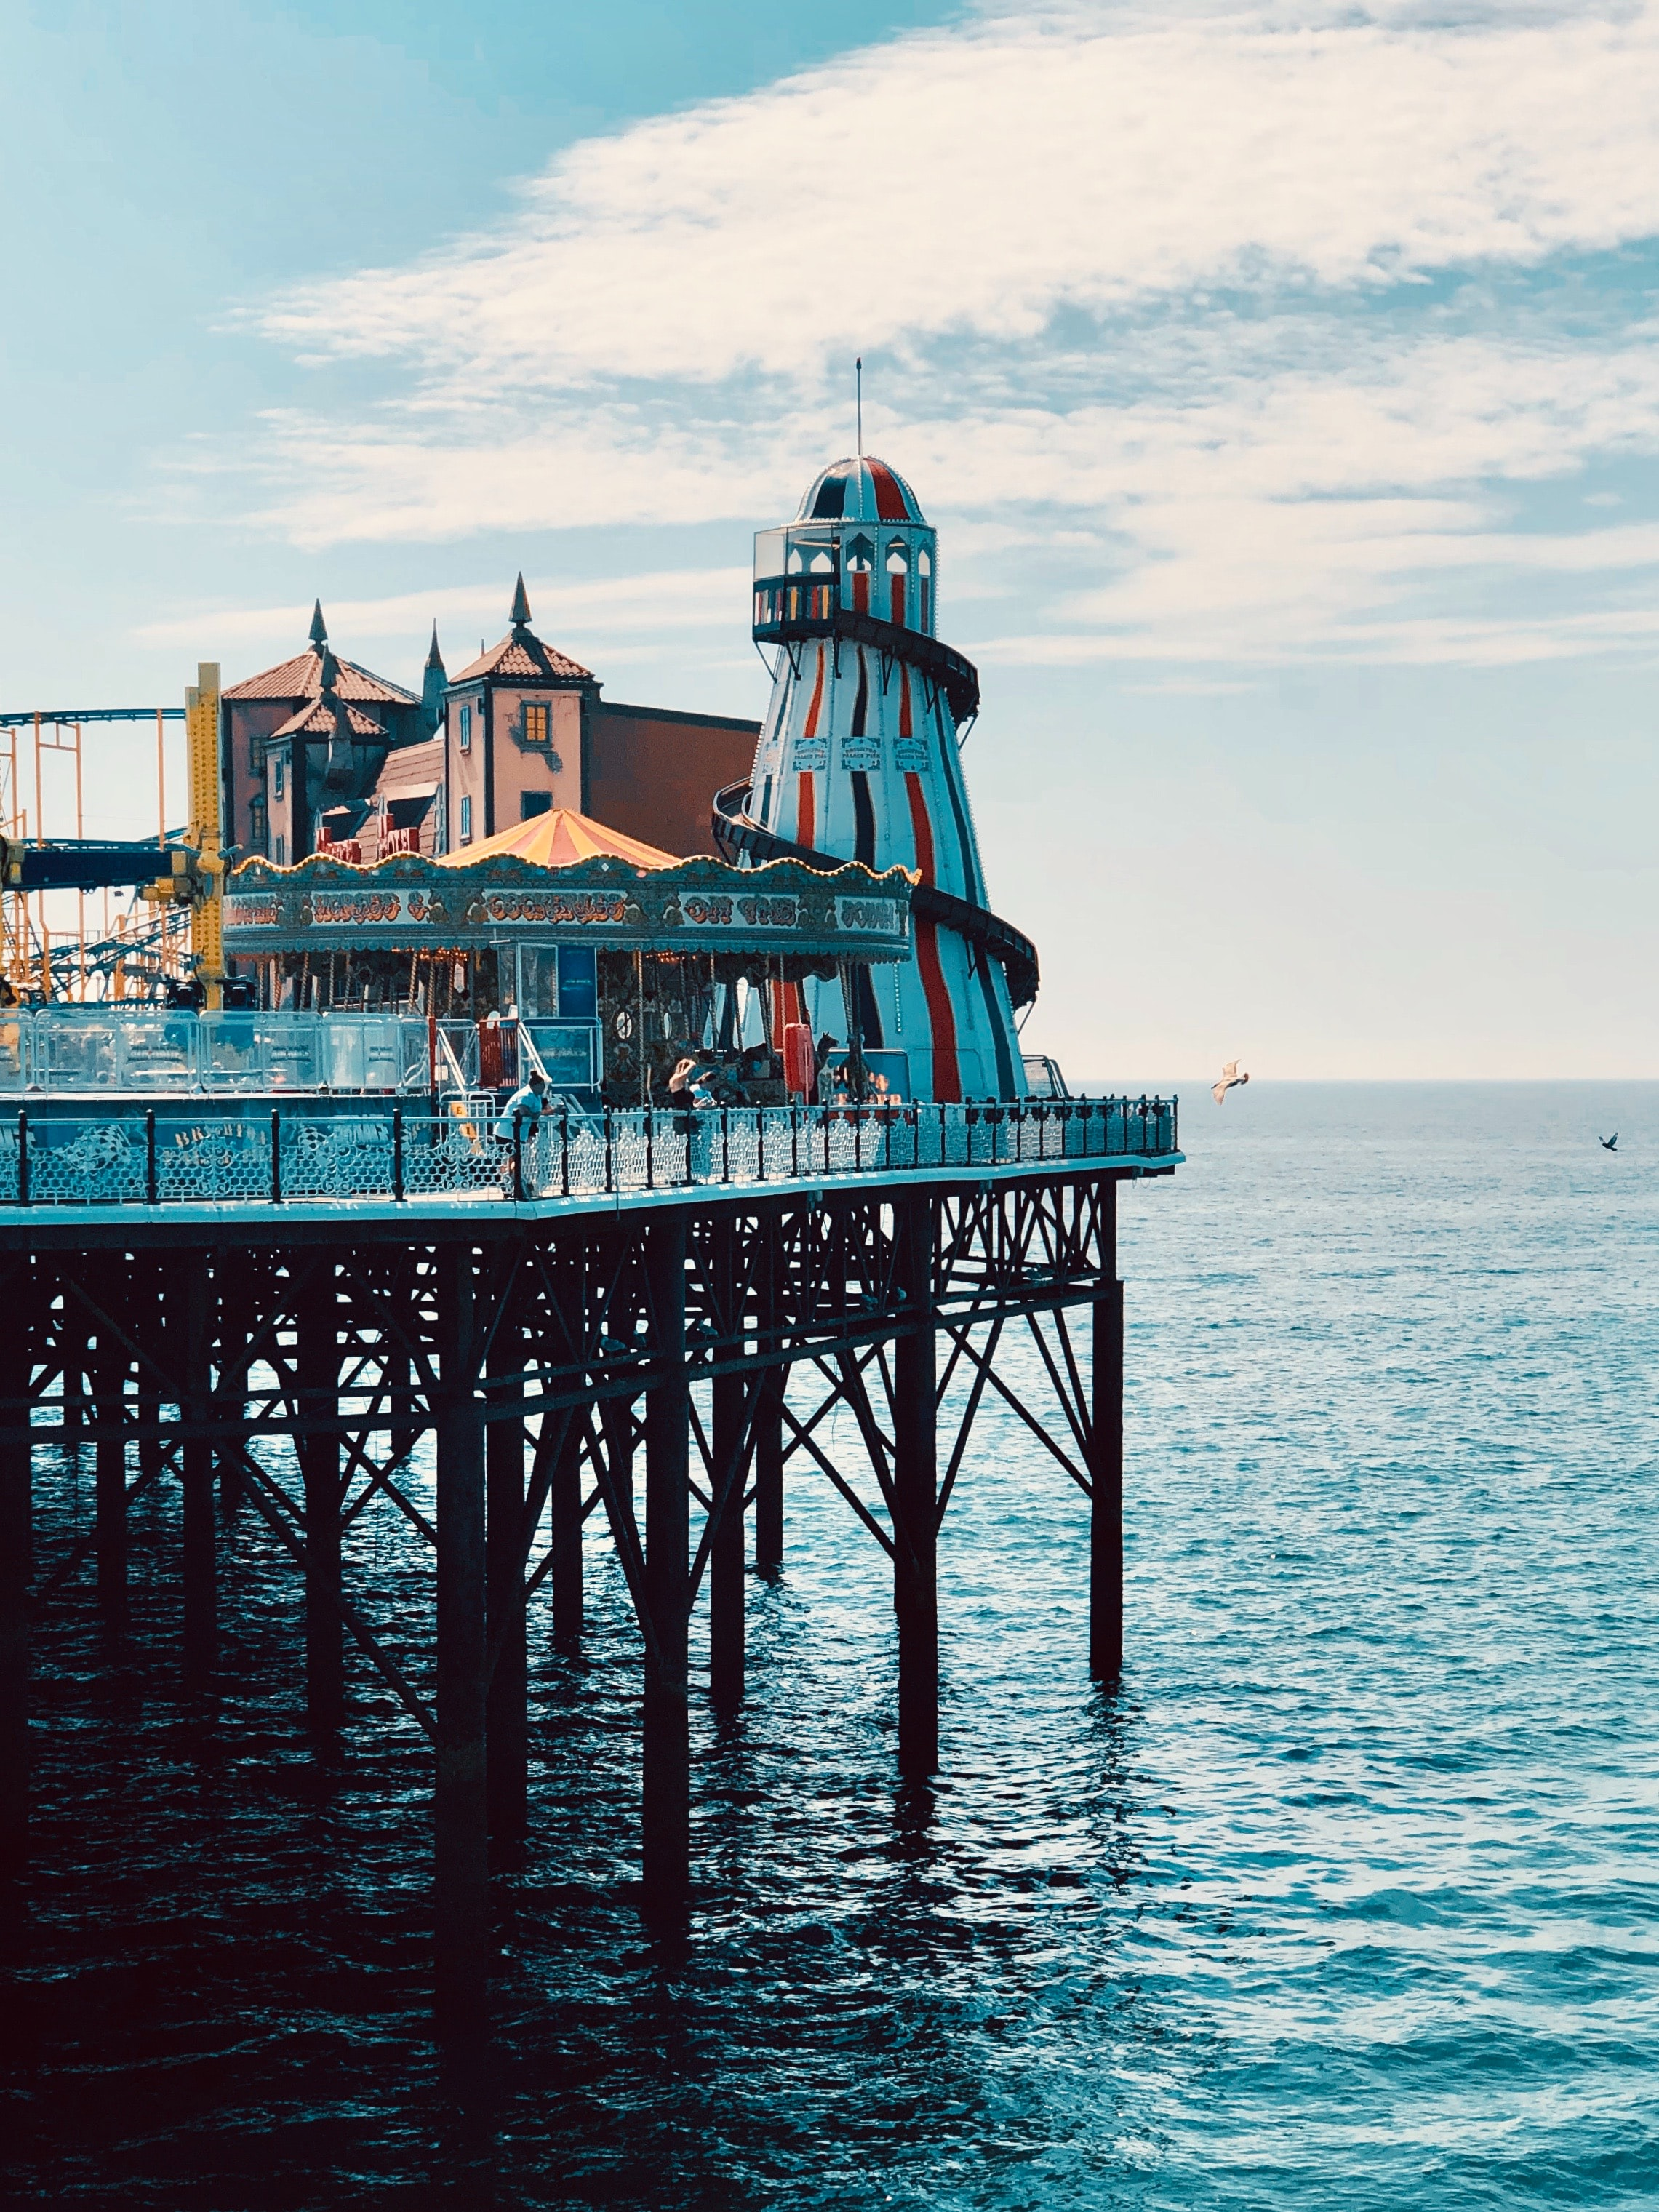
\includegraphics[width=\linewidth]{src/figures/brighton.jpeg}
    \caption{A text-width example.}
    \label{fig:view}
    %% If the optional argument in the square brackets is "none", then the caption *will not appear in the main figure at all* and only the full caption will appear under the supplementary figure at the end of the manuscript.
    \figsupp[Shorter caption for main text.]{This is a supplementary figure's full caption, which will be used at the end of the manuscript.}{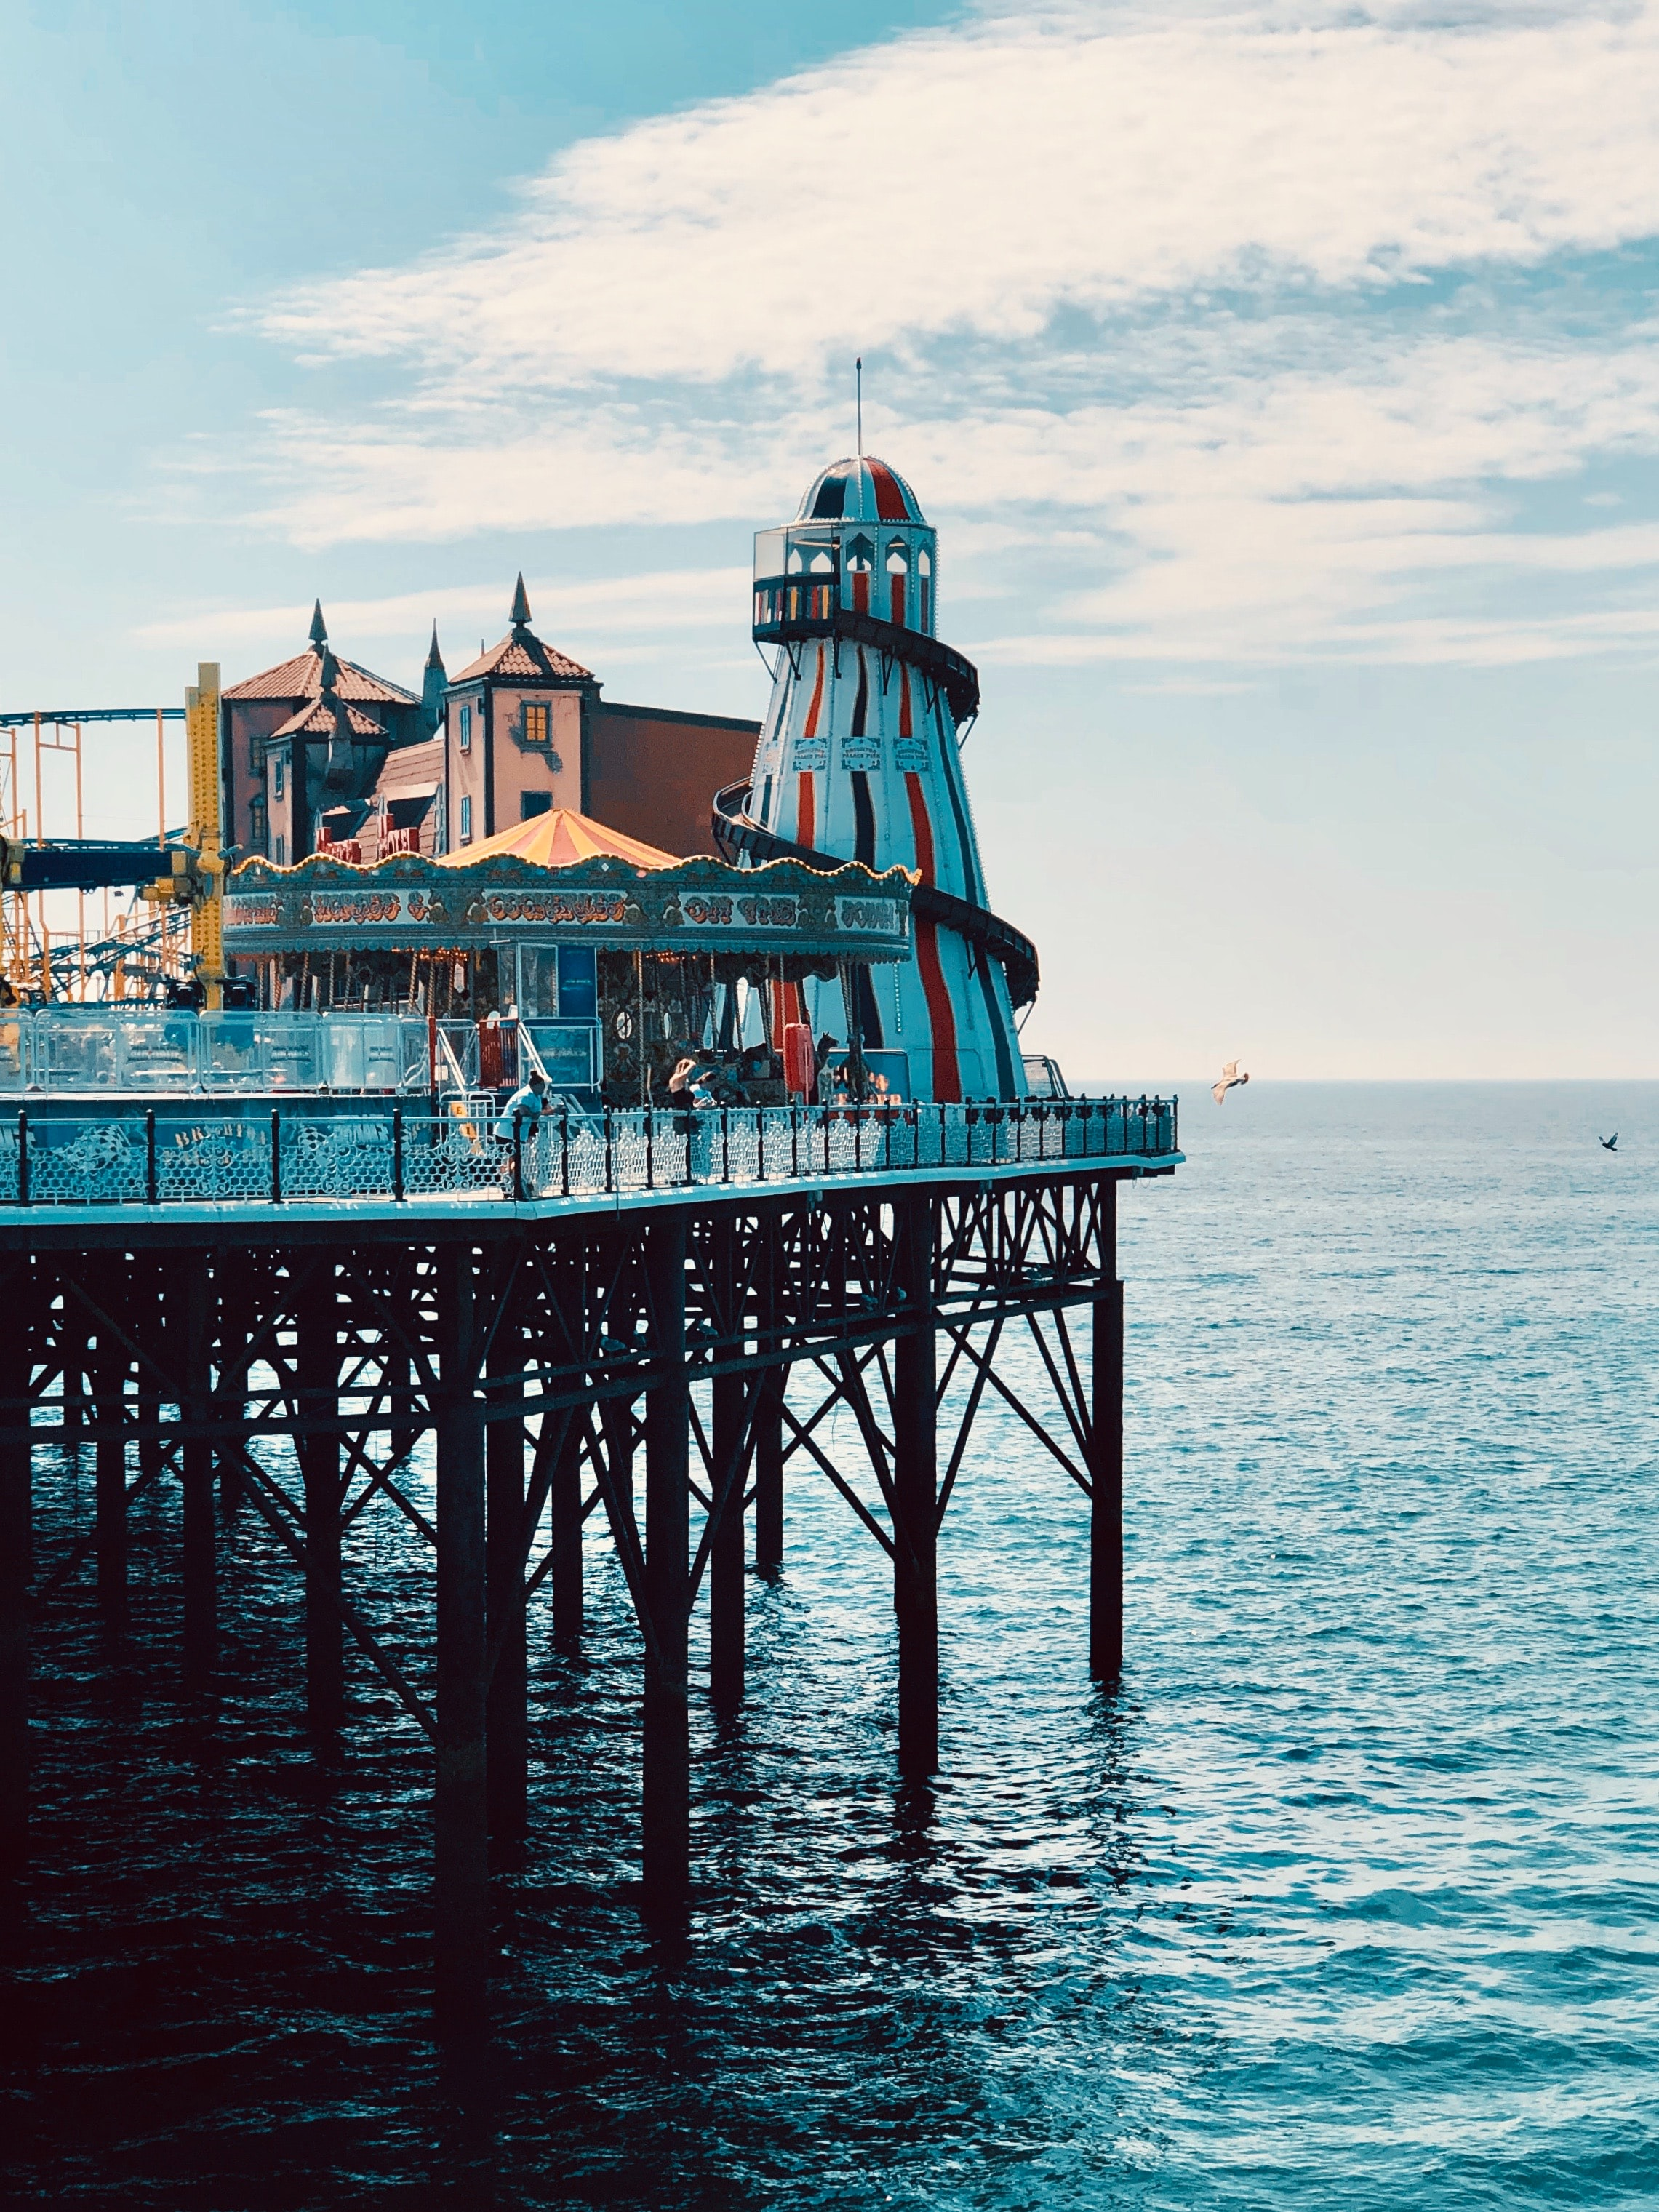
\includegraphics[width=6cm]{src/figures/brighton}}\label{figsupp:sf1}
    \figsupp{This is another supplementary figure.}{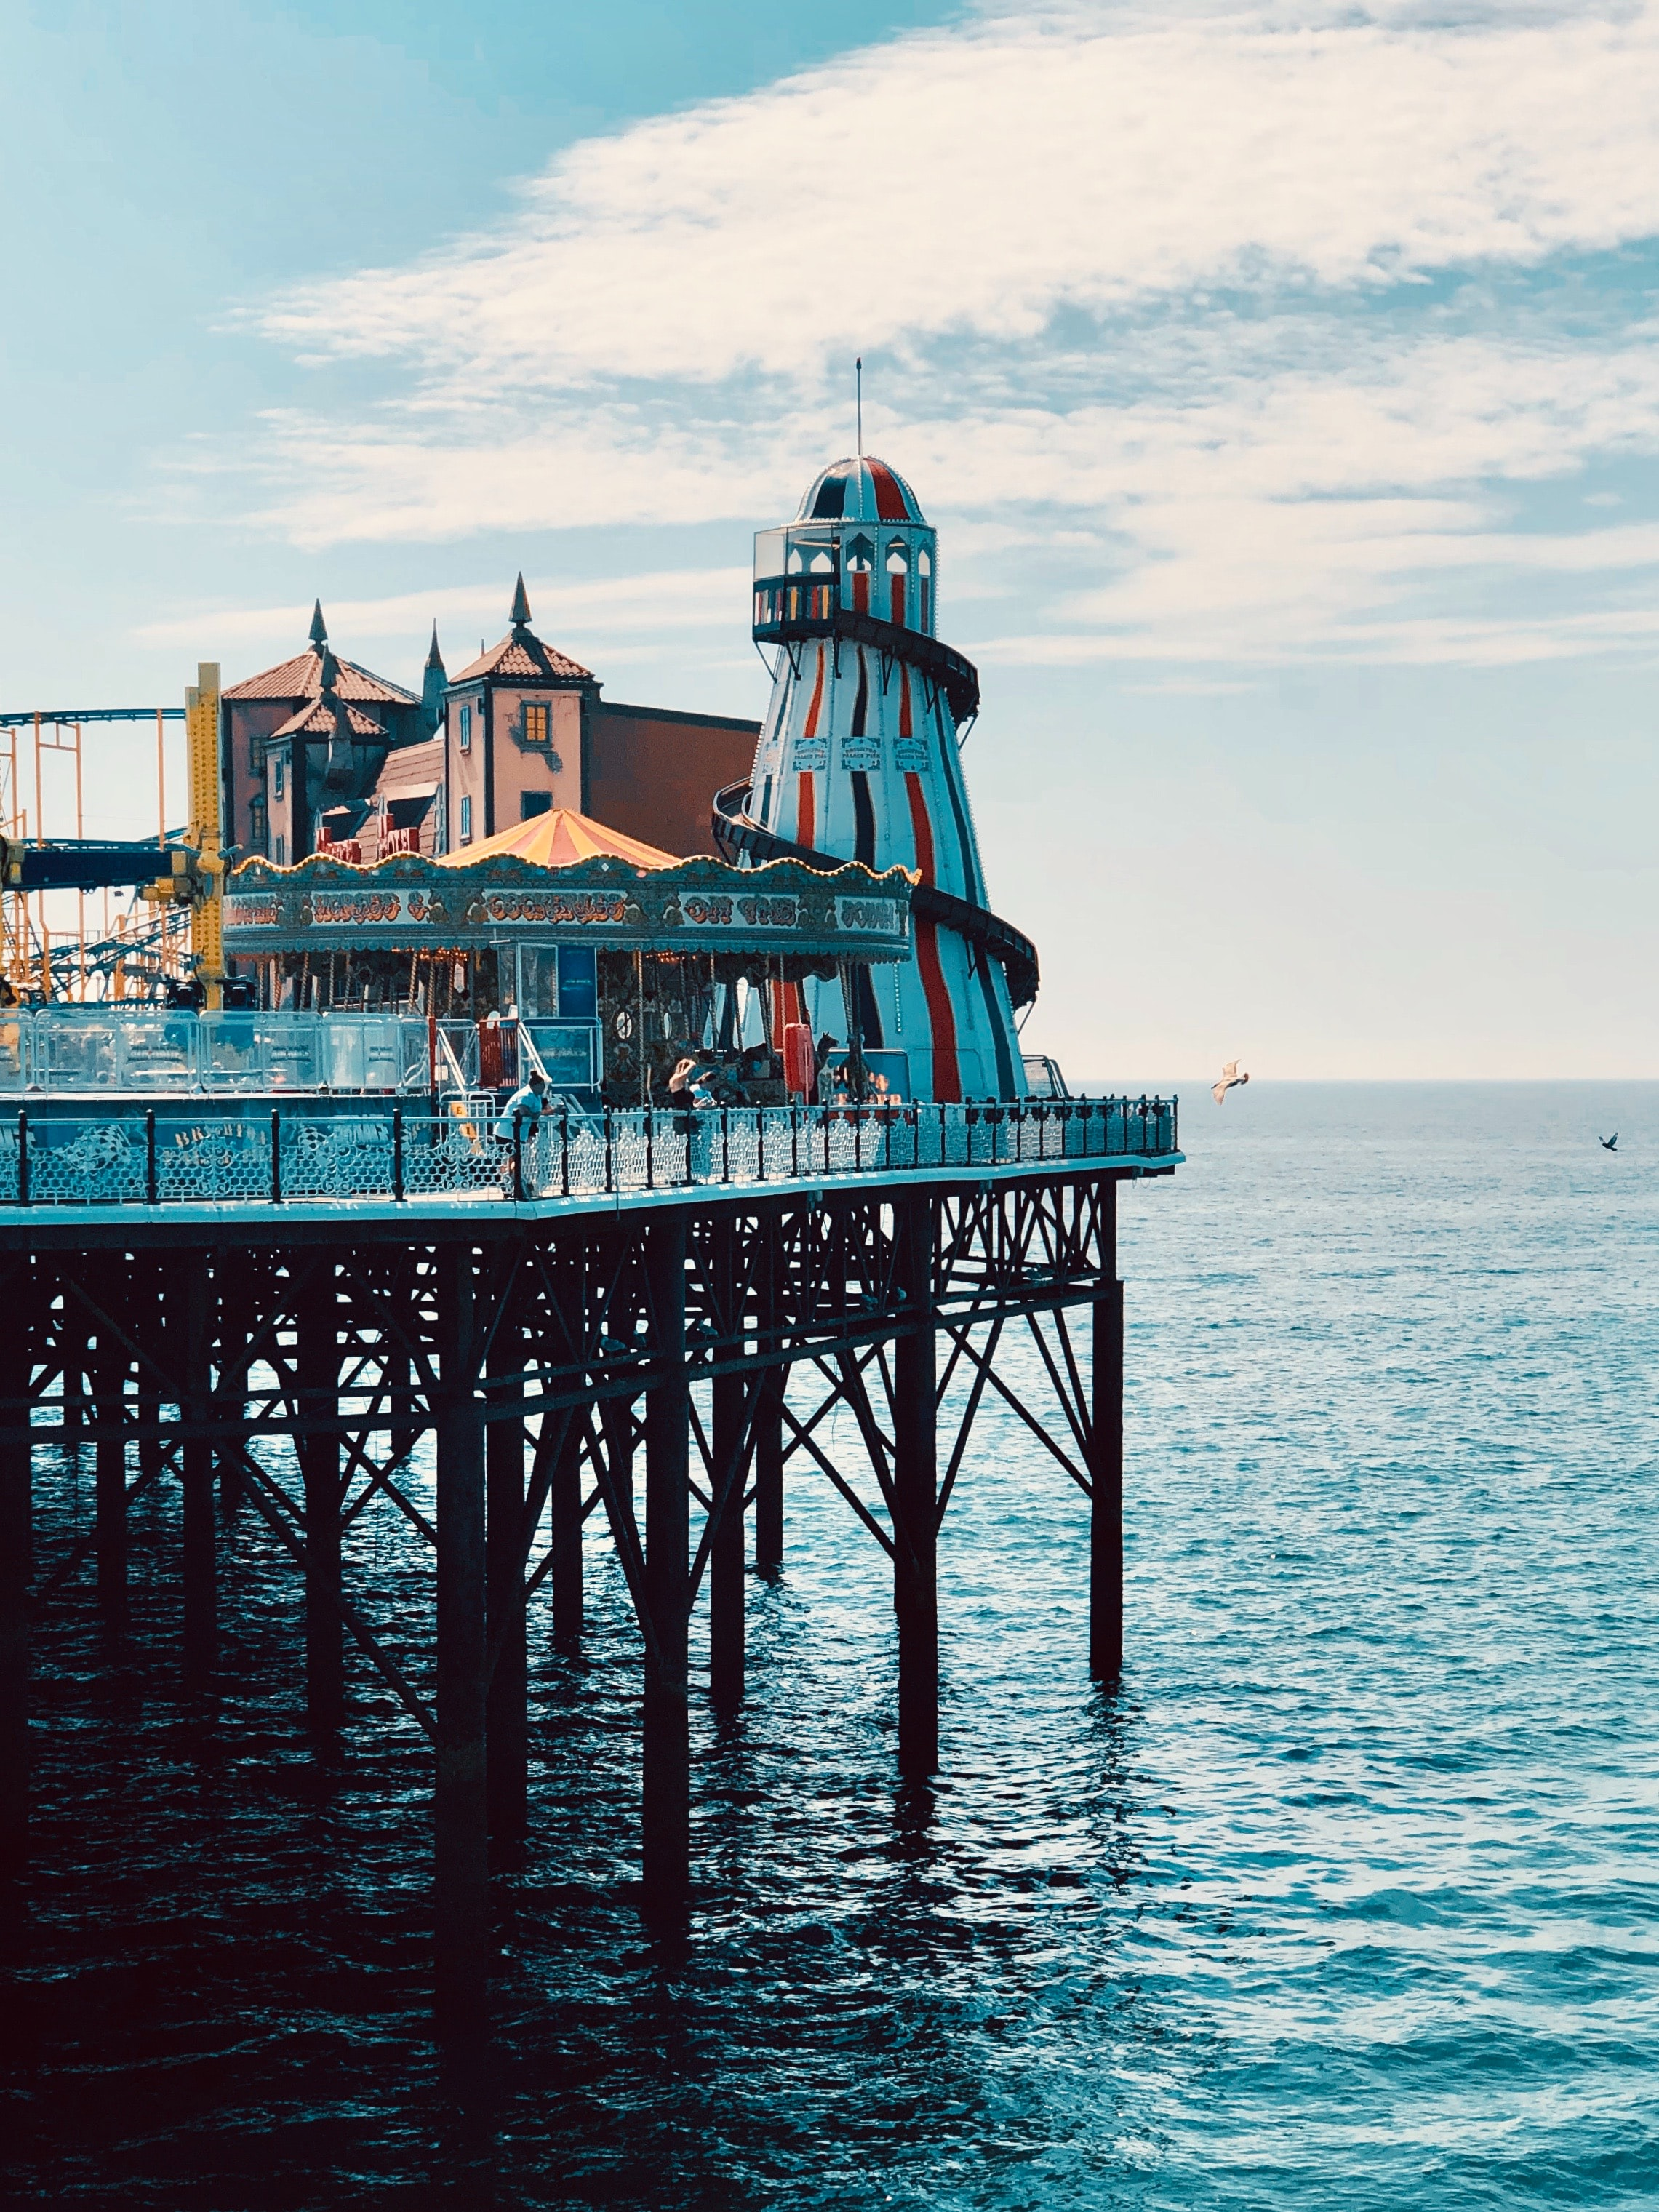
\includegraphics[width=6cm]{src/figures/brighton}}
    \videosupp{This is a description of a video supplement.}\label{videosupp:sv1}
    \figdata{This is a description of a data source.}\label{figdata:first}
    \figdata{This is another description of a data source.}\label{figdata:second}
    \figsrccode{This is a description of a source code.}\label{figsrccode:first}
\end{figure}

\subsection{Other Chemistry Niceties}

You can use commands from the \texttt{mhchem} and \texttt{siunitx} packages. For example: \ce{C32H64NO7S}; \SI{5}{\micro\metre}; \SI{30}{\degreeCelsius}; \SI{5e-17}{\Molar}

\subsection{Lists}

You can make lists with automatic numbering \dots

\begin{enumerate}
    \item Like this,
    \item and like this.
\end{enumerate}
\dots or bullet points \dots
\begin{itemize} 
    \item Like this,
    \item and like this.
\end{itemize}
\dots or with words and descriptions \dots
\begin{description}
    \item[Word] Definition
    \item[Concept] Explanation
    \item[Idea] Text
\end{description}

Some filler text, because empty templates look really poorly. \lipsum[1]

\section{Examples} \label{examples}

\subsection{Downloading data for a gene}

Curated HLA genotype data is provided by the IMGT/HLA database at \href{https://github.com/ANHIG/IMGTHLA}{GitHub}.
In the example below, we use \textit{hlabud} to download the sequence alignment data for \textit{HLA-DRB1}, read it into R, and encode it as a one-hot matrix:

\begin{verbatim}
a <- hla_alignments("DRB1")    
\end{verbatim}


With one line of code, \textit{hlabud} will:

\begin{itemize}
    \item Download data from the IMGT/HLA Github repository.
    \item Cache files in a local folder that supports multiple data releases.
    \item Read the data into matrices and dataframes for downstream analysis.
    \item Create a one-hot encoding of the multiple sequence alignment data.
\end{itemize}

\subsection{Computing a dosage matrix}

Once we have obtained a list of genotypes for each individual (e.g. `"DRB1*04:01,DRB1*05:01"`), we can use \textit{hlabud} to prepare data for fine-mapping regression analysis that will reveal which amino acid positions are associated with a phenotype in a sample of individuals. To calculate the number of copies of each amino acid at each position for each individual, we can run:

\begin{verbatim}
dosage(genotypes, a$onehot)
\end{verbatim}

where \textit{genotypes} is a vector of \textit{HLA-DRB1} genotypes and \textit{a\$onehot} is a one-hot matrix representation of \textit{HLA-DRB1} alleles.
The dosage matrix can then be used for omnibus regression \cite{Sakaue2023} or fine-mapping (i.e. regression with each single position) (figexamples\A).

\subsection{Visualizing alleles in two dimensions}

Visualizing data in a two-dimensional embedding with algorithms like UMAP McInnes2018 can help to build intuition about the relationship between all objects in a dataset.
UMAP accepts the one-hot matrix of HLA alleles as input, and the resulting embedding can be used to visualize the dataset for exploratory data analysis (figexamples\B).

\subsection{Allele frequencies in human populations}

\textit{hlabud} provides direct access to the allele frequencies of HLA genes in the Allele Frequency Net Database (AFND) Gonzalez-Galarza2020 (#link("http://allelefrequences.net")) (figexamples\C).

\subsection{HLA divergence}

Each HLA allele binds a specific set of peptides.
So, an individual with two highly dissimilar alleles can bind a greater number of different peptides than a homozygous individual Wakeland1990.
\textit{hlabud} implements the Grantham divergence calculations Pierini2018 (based on the original Perl code) to estimate which individuals can bind a greater number of peptides (higher Grantham divergence):

\begin{verbatim}
my_genos <- c("A*23:01:12,A*24:550", "A*25:12N,A*11:27", "A*24:381,A*33:85")
hla_divergence(my_genos, method = "grantham")
#> A*23:01:12,A*24:550    A*25:12N,A*11:27    A*24:381,A*33:85 
#>           0.4924242           3.3333333           4.9015152 
\end{verbatim}



\section{Discussion} \label{discussion}

Our open-source R package \textit{hlabud} gives users access to HLA data from two public databases, and implements HLA divergence calculation Pierini2018.
\textit{hlabud} downloads and caches HLA genotype data from the IMGT-HLA GitHub repository imgthla and prepares the data for downstream analysis in R.

We provide \href{https://slowkow.github.io/hlabud}{tutorials} for HLA divergence, fine-mapping association analysis with logistic regression, embedding with UMAP, and visualizing allele frequencies from the Allele Frequency Net Database (AFND) Gonzalez-Galarza2020.

\subsection{Related Work}

BIGDAWG is an R package that provides functions for chi-squared Hardy-Weinberg and case-control association tests of highly polymorphic genetic data like HLA genotypes Pappas2016. HATK is set of Python scripts for processing and analyzing IMGT-HLA data Choi2020.

\subsection{Acknowledgments}

This work was supported by a NIAID grant T32AR007258 (to K.S.) and the National Institute of Health Director’s New Innovator Award (DP2CA247831; to A.C.V.) Thanks to Sreekar Mantena for reporting issues with the code. Thanks to Jean Fan for creating the logo and discussing the paper. 

\subsection{Competing Interests}

No competing interest is declared.

\subsection{Author contributions statement}

K.S. wrote the software and the manuscript. A.C.V. reviewed the manuscript.


\printbibliography

% DON'T EDIT. If "endfloat" option is enabled all floats appear before appendices
\if@endfloat\clearpage\processdelayedfloats\clearpage\fi 


%%%%%%%%%%%%%%%%%%%%%%%%%%%%%%%%%%%%%%%%%%%%%%%%%%%%%%%%%%%%
%%% SUPPLEMENTARY MATERIAL / APPENDICES
%%%%%%%%%%%%%%%%%%%%%%%%%%%%%%%%%%%%%%%%%%%%%%%%%%%%%%%%%%%%
%% Sadly, we can't use floats in the appendix boxes. So they don't "float", but use \captionof{figure}{...} and \captionof{table}{...} to get them properly caption.
%\begin{appendix}

%\begin{appendixbox}\label{app:ttt}
%    \section{TTT, by Piet Hein}
Problems worthy \\
of attack \\
prove their worth \\
by hitting back. \\
\\
Put up in a place \\
where it's easy to see \\
the cryptic admonishment\\
    T.T.T. \\
\\
When you feel how depressingly \\
slowly you climb, \\
it's well to remember that\\
Things Take Time. \\
\\
The road to wisdom? - Well, it's plain\\
and simple to express: \\
   Err \\
   and err \\
   and err again \\ 
   but less \\
   and less \\
   and less. \\

\begin{center}
    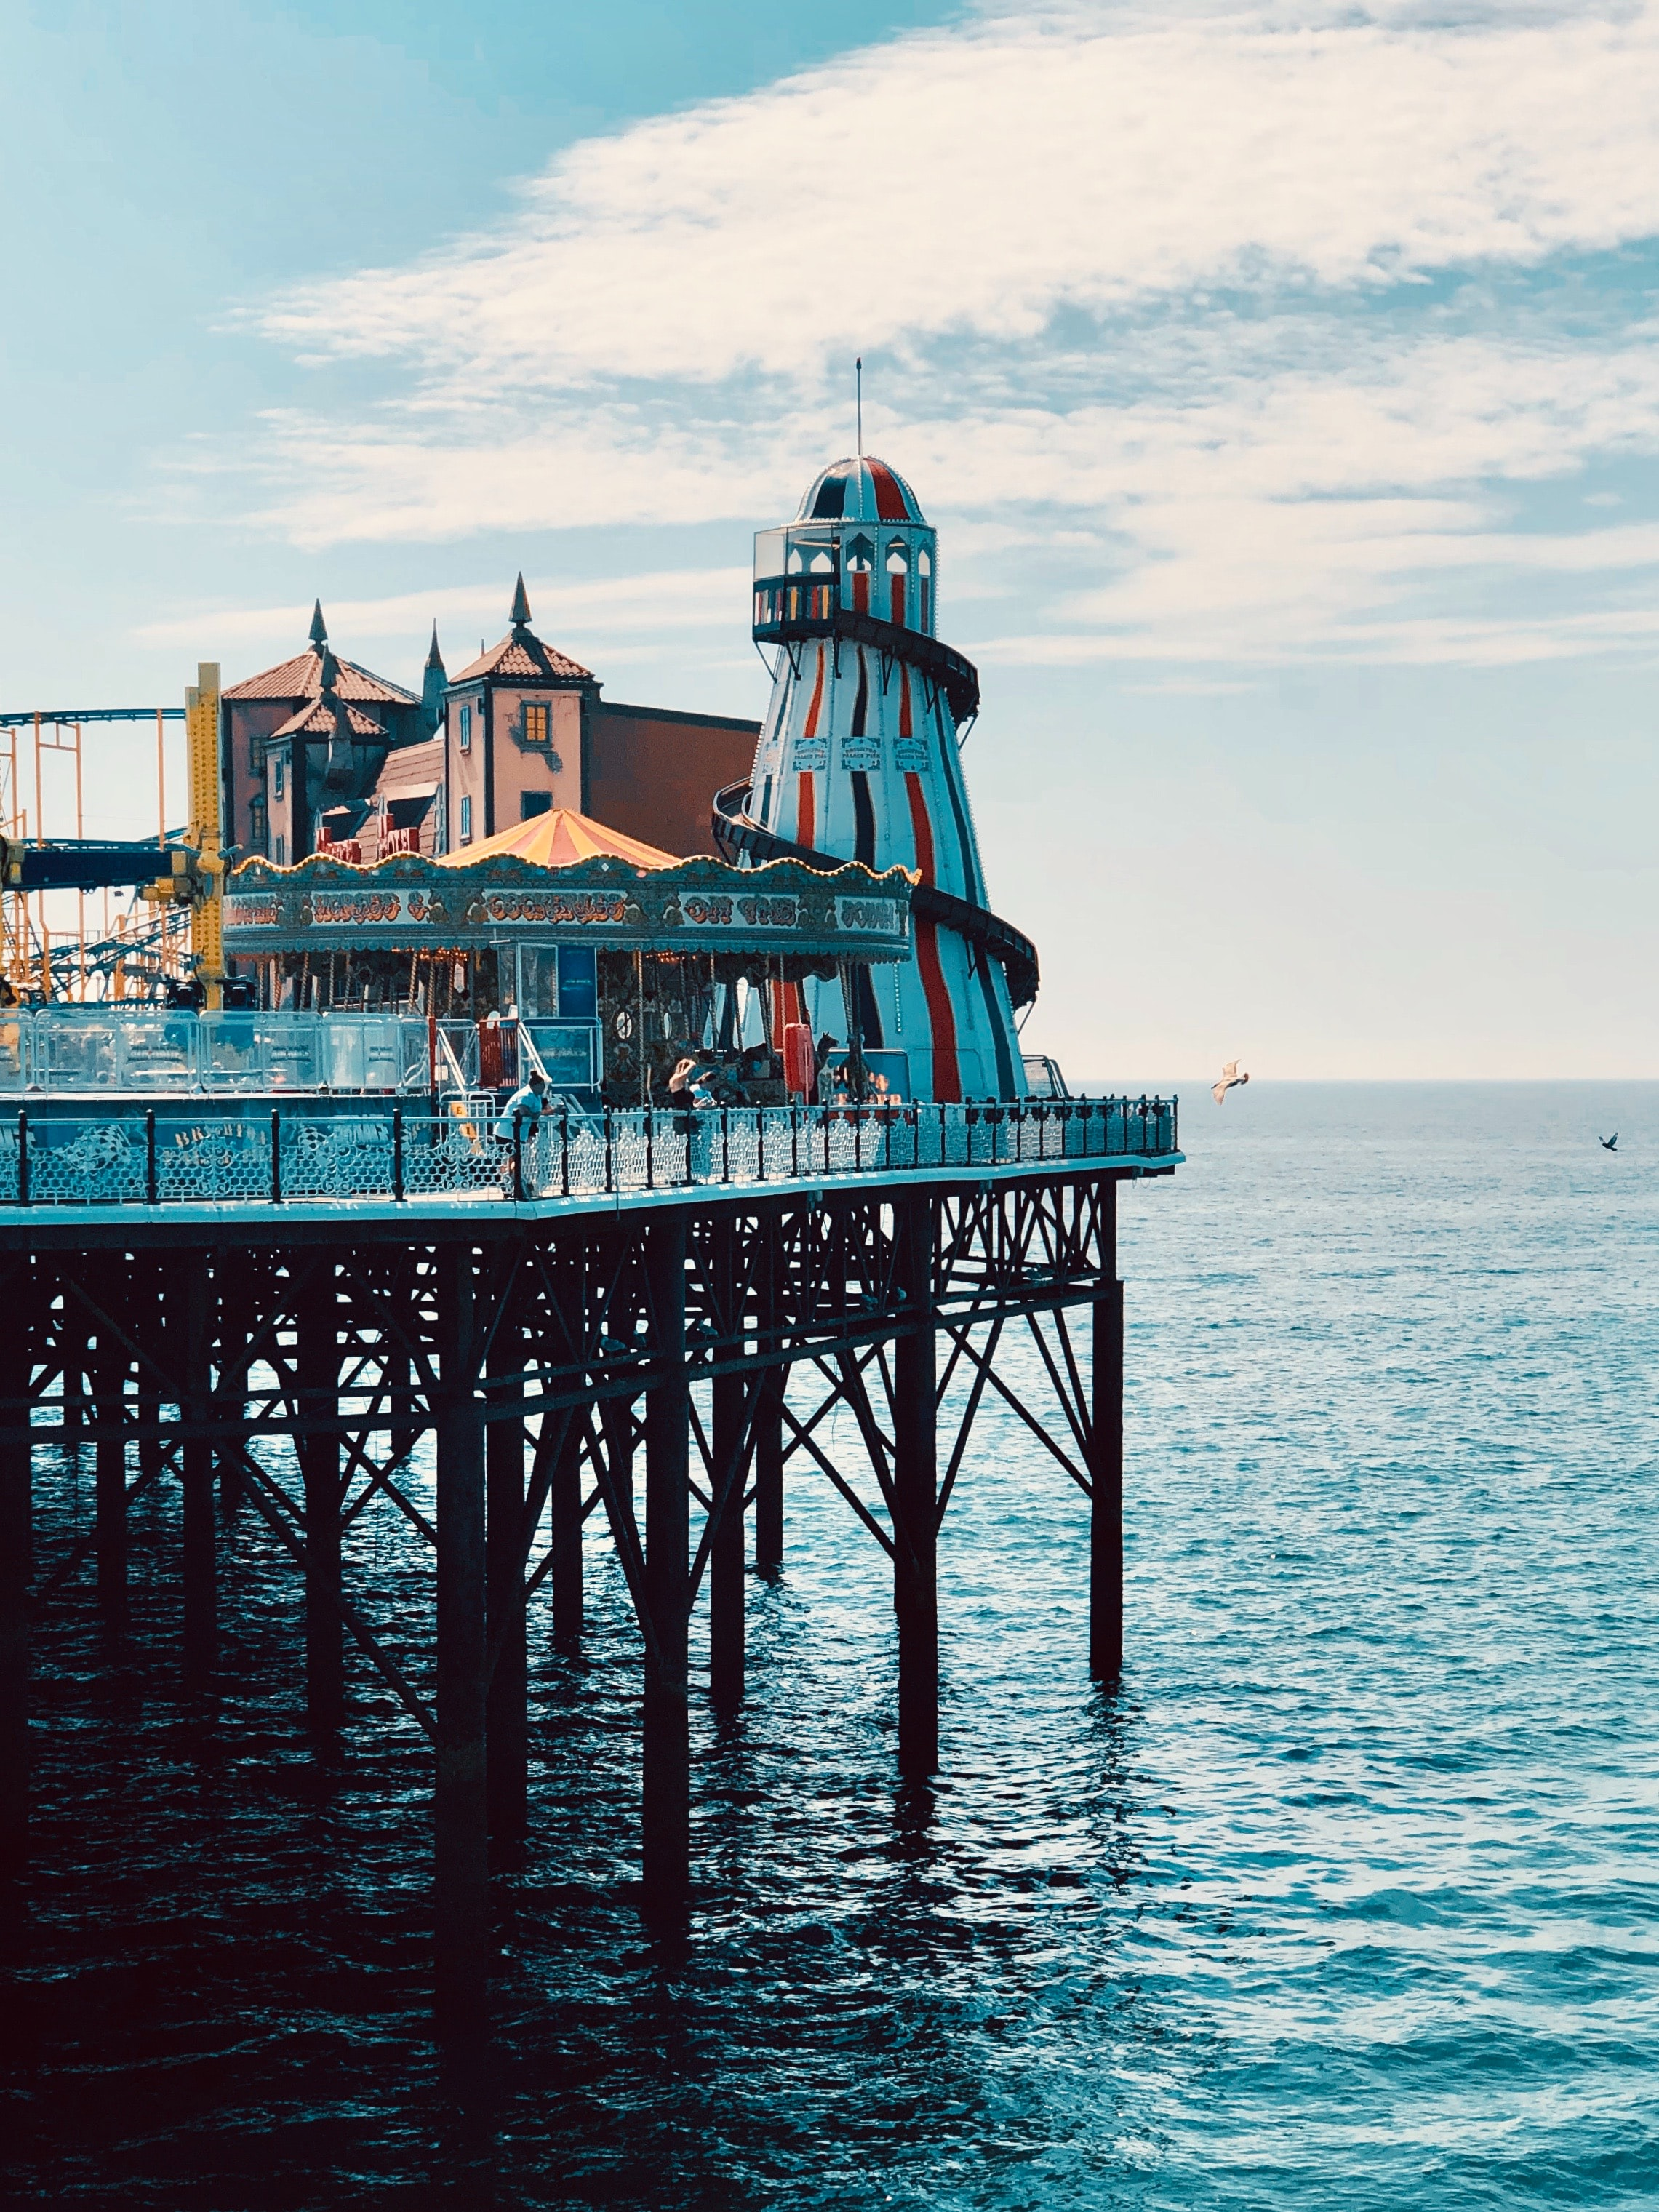
\includegraphics[width=\linewidth,height=7cm]{src/figures/brighton.jpeg}
    \captionof{figure}{This is a figure in the appendix}
\end{center}

%\end{appendixbox}

%\begin{appendixbox}
%    \section{Key resources}
Here could be a nice table of your resources. 

% Make your own table style https://tex.stackexchange.com/questions/94799/how-do-i-color-table-columns
%\end{appendixbox}

%\end{appendix}


%%%%%%%%%%%%%%%%%%%%%%%%%%%%%%%%%%%%%%%%%%%%%%%%%%%%%%%%%%%%
%%% ARTICLE END
%%%%%%%%%%%%%%%%%%%%%%%%%%%%%%%%%%%%%%%%%%%%%%%%%%%%%%%%%%%%

\end{document}
